% !TEX root = mainthesis.tex
%Chapter 5
\externaldocument{Chapter8.tex}

\renewcommand{\thechapter}{5}

\chapter{Fourier Transform Spectroscopy}
\label{ch:Fourier_spectroscopy}


The high level of control in ultracold atomic systems makes them an ideal platform for analog simulation of materials and other complex systems. The properties of these engineered `atomic' materials depend on the underlying single particle energies and it is important to characterize them. We worked on Fourier transform spectroscopy for this purpose. 

Many spectroscopy techniques in atomic physics rely on using 
a source of coherent electromagnetic radiation with a well known frequency that probes the internal structure of a system (atom). For example, in absorption spectroscopy~\cite{demtroder_doppler-limited_2008} coherent light is sent through an atomic medium and if the frequency of the light is resonant with an atomic transition it is absorbed and a reduced transmission is measured. Other variants of spectroscopy (e.g. Rabi spectroscopy~\cite{rabi_space_1937}, spin-injection spectroscopy~\cite{cheuk_spin-injection_2012}) work under a similar principle: atoms absorb and emit photons with frequencies equal to the transition energies between internal states. 

Fourier transform spectroscopy instead employs the connection between the energy spectrum of a system and its dynamics. This connection has been exploited to study the spectrum of both condensed matter \cite{jonas_two-dimensional_2003} and cold atom systems \cite{yoshimura_diabatic-ramping_2014,wang_atom-interferometric_2015} alike.
As opposed to other techniques, Fourier spectroscopy relies only on following the unitary evolution of an initial state suddenly subjected to a Hamiltonian of interest and measuring probabilities in a basis that does not diagonalize that Hamiltonian. 
% This spectroscopic tool is also useful for studying the energy spectrum of more complex time-dependent periodically driven systems \cite{eckardt_superfluid-insulator_2005,goldman_periodically_2014}, which are well suited for engineering and tuning Hamiltonians.

The frequency resolution of Fourier transform spectroscopy is limited only by the coherent evolution timescale of the system under study and can otherwise be applied to any system. Other applications of this technique implemented in our laboratory that are not included in this Chapter include measuring the dispersion relation of a Rashba spin-orbit coupled gas (see Chapter~\ref{ch:Rashba}) and the band structure of a fractional period adiabatic superlattice~\cite{anderson_realization_2019}.

This Chapter is organized as follows: First, I give a general description of the Fourier transform spectroscopy technique in Section~\ref{sec:fs-theory}. In Section~\ref{sec:fs-exp} I describe a set of experiments where we engineered a tunable spin-orbit coupled system and applied Fourier transform spectroscopy. This work was published in~\cite{valdes-curiel_fourier_2017}.

% which offers the advantage of simultaneous recording
% of a large spectral interval and with it a short measuring time.

\section{Operating principle of Fourier spectroscopy}
\label{sec:fs-theory}
%
\begin{figure*}[!ht]
	\begin{center}
		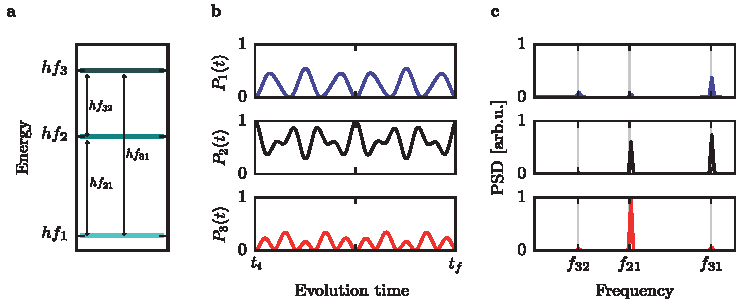
\includegraphics{Figures/Chapter5/Fig1.pdf}
		\caption[Operating principle of Fourier spectroscopy]
		{
			{\bf a.} Eigenenergies of a three-level system described by $\hat{H}'(\Omega_1,\Omega_2,\Omega_3)$. 
			{\bf b.} The system is prepared in $\ket{\psi_2}$ and subjected to $\hat{H}'$ at time $t_i$. The three panels show the occupation probabilities of the states $\ket{\psi_1}$ (blue), $\ket{\psi_2}$ (black), and $\ket{\psi_3}$ (red) in the measurement basis, for evolution times up to $t_f$. 
			{\bf c.} Power spectral density of the occupation probabilities from panel b. The three peaks in the Fourier spectra correspond to the energy differences present in panel a.
		\label{fig:Figure1}}
	\end{center}
\end{figure*}
%
We focus on a system where we can measure the occupation probabilities of a set of orthonormal states $\{\ket{\psi_i}\}$ that fully span the accessible Hilbert space of the system. We then consider the time evolution of an arbitrary initial state $\ket{\Psi_0}=\sum\limits_{i}a_i\ket{\psi_i}$ as governed by a Hamiltonian $\hat{H}'(\{\Omega_i \})$ and observe the occupation probabilities of the $\{\ket{\psi_i}\}$ states of the measurement basis as a function of time. When $\hat{H}'$ is applied, the evolution of the initial state is $\ket{\Psi(t)}=\sum\limits_{i,j}a_ic_{i,j}e^{-iE'_jt/\hbar}\ket{\psi'_j}$, where $E'_j$ and $\ket{\psi'_j}$ are the eigenenergies and eigenstates of $\hat{H}'$, and $c_{i,j}(t)=\braket{\psi_i}{\psi'_j}$. The probability 
%
\begin{align}
P_k(t)=&|\braket{\psi_k}{\Psi(t)}|^2=\lvert\sum\limits_{i,j}a_ic_{i,j}c^{*}_{j,k}e^{-iE'_jt/\hbar}\rvert^2
\label{Eq:Probability}
\end{align}
%
of finding the system in a state $\ket{\psi_k}$ of the measurement basis can be expressed as a sum of oscillatory components, with amplitude given by the magnitude of the overlap integrals between the initial state and the eigenvalues of $\hat{H}'$
\begin{align}
%P_k(t)=\tilde{a}_k+\sum\limits_{i\neq j}\tilde{b}_{i,j,k}\cos(2\pi f_{j,j'}t),
P_k(t)=1+\sum\limits_{i,j\neq l} 2\lvert a_i^2c_{i,j}c_{j,k}c_{i,l}c_{l,k}\rvert \cos(2\pi f_{j,l}t),
\end{align}
where $f_{j,l}=(E'_{j}-E'_{l})/h$ is the frequency associated with the energy difference of two eigenstates of the Hamiltonian.
Fourier spectroscopy relies on measuring the populations on each state of the measurement basis as a function of time and extracting the different frequency components $f_{j,l}$ directly by computing the discrete Fourier transform. The bandwidth and frequency resolution of the measurement are determined by the total sampling time and the number of samples. For $N$ samples separated by a time interval $\Delta t$, the highest resolved frequency will be $f_{\mathrm{bw}}=1/2\Delta t$, with resolution $\Delta f=1/\Delta tN$. This resolution can be decreased if the Fourier transform is calculated using certain types of windowing functions that enhance signal to noise ratio.  Any  higher frequency  $f>f_{\mathrm{bw}}$ will be aliased and measured in the Fourier spectrum as $f_{\mathrm{alias}}=\vert f - m/\Delta t \vert$, where $m$ is an integer. If interactions are present in the system, the dynamics get modified in a time scale given by the magnitude of the interactions, giving an additional constraint to the smallest frequency components of a single particle Hamiltonian that can be resolved with our technique.

Figure~\ref{fig:Figure1} illustrates the principle of Fourier spectroscopy for a three level system, initially prepared in the state $\ket{\Psi_0}=\ket{\psi_2}$, subject to the Hamiltonian
%
\begin{equation}
\hat{H}'=\begin{pmatrix}
E_1 & 0 & 0  \\
0 & E_2 & 0  \\
0 & 0 & E_3 \\
\end{pmatrix}
+\hbar\begin{pmatrix}
0 & \Omega_1 & \Omega_2  \\
\Omega_1^{*} & 0 & \Omega_3  \\
\Omega_2^{*} & \Omega_3^{*} & 0
\end{pmatrix},
\end{equation}
%
where we measure the occupation probability as a function of time for each of the $\{\ket{\psi_1}, \ket{\psi_2},\ket{\psi_3}\}$ states. The three eigenenergies $E'_i=hf_i$ that result from diagonalizing $\hat{H}'$are displayed in Figure~\ref{fig:Figure1}a. The three energy differences $hf_{jj'}$ between the levels determine the oscillation frequencies of the occupation probabilities, as can be seen in Figure~\ref{fig:Figure1}b. Finally, Figure~\ref{fig:Figure1}c shows a plot of the power spectral densities (PSD) with three peaks corresponding to the three relative energies of $\hat{H}'$. 
%
\section{Measuring the SOC dispersion with Fourier transform spectroscopy}
\label{sec:fs-exp}

We applied the Fourier transform spectroscopy technique to measure the dispersion relation of spin-1 BECs with an equal superposition of Rashba and Dresselhaus SOC, and tunable SOC strength.

\subsection{System}

\sloppy All of our experiments started with BECs containing about $4\times 10^4$ atoms in the $\ket{f=1,m_F=-1}$ hyperfine state. The experiments described in Section~\ref{sec:application_of_fs} were performed in an optical dipole trap with frequencies $(\omega_x,\omega_y,\omega_z)/2\pi=(42(3),34(2),133(3))\Hz$. We later modified the trapping frequencies in the $xy$ plane to try to make them more symmetric for the experiments described in Section~\ref{sec:effective_mass}. We broke the degeneracy of the three $m_F$ magnetic sub-levels by applying a $1.9893(3)\,$mT bias field along $\mathbf{e}_z$ that produced a $\omega_Z / 2\pi  = 14.000(2) \MHz$ Zeeman splitting, and a quadratic Zeeman shift $\epsilon$ that shifted the energy of $\ket{f=1,m_F=0}$ by $-h\times (28.45\, \kHz)$. We transfered atoms into the $\ket{f=1,m_F=0}$ state using ARP (see Section~\ref{sec:arp}) and then we monitored and stabilized the magnetic field using partial transfer absorption imaging  (Section~\ref{sec:ptai}) by applying a pair of $\unit[250]{\mu s}$ microwave pulses, each of them detuned by $\pm \unit[2]{kHz}$ from the $\ket{f=1, m_F=0}\leftrightarrow\ket{f=2, mf=1}$ transition.

\begin{figure*}[!ht]
	\begin{center}
		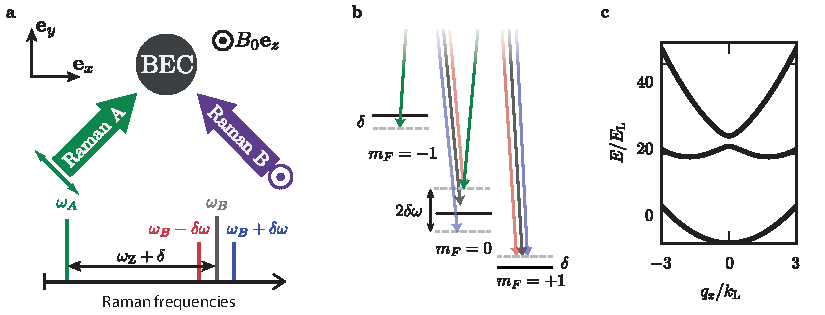
\includegraphics{Figures/Chapter5/Fig2.pdf}
		\caption[Experimental setup for engineering a tunable system with equal contributions of Rashba and Dresselhaus-type spin-orbit coupling]
		{
			{\bf a.} Setup. A bias magnetic field $B_0\ez$, with $B_0=1.9893$\,mT splits the hyperfine energy levels of the $f=1$ manifold of $^{87}$Rb by $\omega_Z/2\pi=14$\,MHz. A pair of cross polarized Raman beams propagating along $\ex+\ey$ and $\ex-\ey$ couple the atoms' momentum and spin states. 
			{\bf b.} The Raman frequencies are set to $\omega_A=\omega_L+\delta$ and $\omega_B=\omega_L+\omega_Z$. We add frequency sidebands to $\omega_B$, separated by $\pm \delta\omega$. The amplitude modulation from the interference between the multiple frequency components results in tunable SOC.
			{\bf c.} SOC dispersion for Raman coupling strength $\Omega_0=12E_{\mathrm{L}}$ and $\Omega=0$, on four photon resonance.
		\label{fig:Figure2}}
	\end{center}
\end{figure*}

We induced spin-orbit coupling using a pair of intersecting, cross polarized Raman laser beams propagating along $\mathbf{e}_x+\mathbf{e}_y$ and $\mathbf{e}_x-\mathbf{e}_y$, as shown in Figure~\ref{fig:Figure2}a and b. The beams had angular frequency $\omega_A=\omega_L+\delta$ and $\omega_B=\omega_L+\omega_Z$, where $2\delta$ is the, experimentally controllable, detuning from four photon resonance between $m_F=-1$ and $m_F=+1$. 

Our system was well described by the Hamiltonian including atom-light interaction along with the kinetic contribution
 
 \begin{align}
 \begin{split}
 \hat{H}_{\mathrm{SOC}} = &\frac{\hbar^2q_x^2}{2m} + \alpha q_x\hat{F}_z  + 4E_{\mathrm{L}}\hat{\mathbb{1}} + \hbar\Omega_{\mathrm{R}}\hat{F}_x  +(4E_{\mathrm{L}}-\epsilon)(\hat{F}_z^2-\hat{\mathbb{1}}) +\hbar\delta\hat{F}_z,
 \label{Eq:SOCone}
 \end{split}
 \end{align}
 %
where $q$ is the quasimomentum, $\hat{F}_{x,y,z}$ are the spin-1 angular momentum matrices,  $\alpha=\hbar^2k_{\mathrm{L}}/m$ is the SOC strength, and $\Omega_{\mathrm{R}}$ is the Raman coupling strength, proportional to the Raman laser intensity. The Raman field coupled $\ket{m_F=0,\, q=q_x}$ to $\ket{m_F=\pm1,\, q=q_x\mp 2k_{\mathrm{L}}}$, generating a spin change of $\Delta m_F=\pm1$ and imparting a $\mp 2k_{\mathrm{L}}$ momentum. The eigenstates of $\hat{H}_{\mathrm{SOC}}$ were linear combinations of these states and $\ket{m_F=0,\,q=q_x}$, and the set $\{\ket{m_F,q}\}$ constituted the measurement basis for Fourier transform spectroscopy.

Figure \ref{fig:Figure2}c shows a typical band structure of our spin-1 SOC system as a function of quasimomentum for a large and negative quadratic Zeeman shift $-\epsilon>4E_{\mathrm{L}}$. In this parameter regime, the ground state band had a nearly harmonic dispersion with an effective mass $m^{*} = \hbar^2[d^2E(k_x)/d^2x]^{-1}$, only slightly different from that of a free atom. 

\subsection{Tunable SOC}
We engineered a highly tunable dispersion relation in which we could independently control the size of the gap at $q_x=0$ as well as the SOC strength $\alpha$ by adding frequency sidebands to one of the Raman beams. The state of the system could change from $\ket{m_F=-1,\,q=q_x+2k_{\rm{L}}}$ to  $\ket{m_F=1,\,q=q_x-2k_{\mathrm{L}}}$ by absorbing a red detuned photon first followed by a blue detuned photon and vice versa, in a similar way to the M\o lmer-S\o rensen entangling gate in trapped ion systems \cite{sorensen_entanglement_2000}. When we set the angular frequencies of the sidebands to $\omega=\omega_{\mathrm{A}}+\omega_Z \pm \delta\omega$, the Hamiltonian (Equation~\ref{Eq:SOCone}) acquired a time-dependent coupling $\Omega_{\mathrm{R}}(t)=\Omega_0 + \Omega\cos(\delta\omega t)$. This periodically driven system was well described by Floquet theory \cite{floquet_sur_1883} (see Section~\ref{sec:Floquet_theory}). Figure~\ref{fig:Floquet} shows the spectrum of Floquet quasi-energies for a system described by Equation~\ref{Eq:SOCone} where $\Omega_{\rm R}$ oscillated with angular frequency $\delta\omega$. 
%
\begin{figure*}[htb]
	\begin{center}
		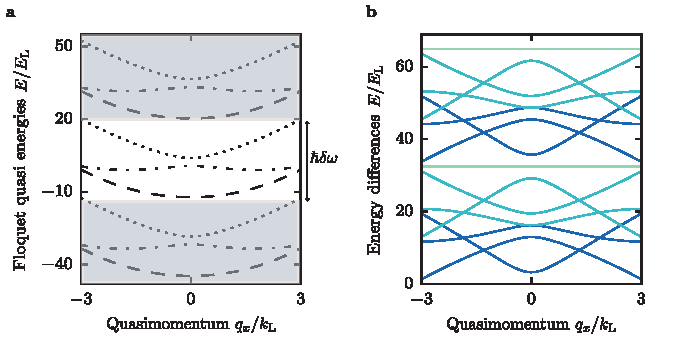
\includegraphics{Figures/Chapter5/Fig3.pdf}
		\caption[Floquet quasi-energy spectrum of a three-level system with spin-orbit coupling and periodic coupling strength]
		{
			{\bf a.} Floquet quasi-energies of a three level Hamiltonian with SOC and time periodic coupling strength. The quasi-energies are grouped into manifolds consisting of three levels that get repeated with a periodicity equal to $\hbar\delta\omega$.
%
			{\bf b.} Energy differences of the Floquet quasi-energies. Each color represents the energy difference, separated by a fixed number of neighboring levels. When the number of neighboring levels is a multiple of 3, the energy differences are straight lines, a result of the periodic structure of the Floquet manifolds. 
		\label{fig:Floquet}}
	\end{center}
\end{figure*}

We found an effective time-independent Hamiltonian using a unitary transformation $\hat{U}(t)$ and applying a RWA. The time evolution of the transformed wave function  $\ket{\psi'}=\hat{U}^{\dag}\ket{\psi}$ was given by the time dependent Schr\"odinger equation for the Hamiltonian $\hat{H}'=\hat{U}^{\dag}\hat{H}\hat{U}-i\hbar\hat{U}^{\dag}\partial_t\hat{U}$. We used 
\begin{equation}
\hat{U}(t)=\mathrm{exp}[-i\frac{\Omega}{\delta\omega}\sin(\delta\omega t)\hat{F}_x]
\end{equation}
%
\sloppy so that $i\hbar\hat{U}^{\dag}\partial_t\hat{U}=\hbar\Omega_{\rm R}(t)\fx$. The transformed Hamiltonian $\hat{H}'(t)$ had terms proportional to $\sin(\Omega/\delta\omega\sin(\delta\omega t))$, $\sin^2(\Omega/\delta\omega\sin(\delta\omega t))$, $\cos(\Omega/\delta\omega\sin(\delta\omega t))$ and $\cos^2(\Omega/\delta\omega\sin(\delta\omega t))$ which we simplified using the Jacobi-Anger expansion
\begin{align*}
&\cos(z\sin\theta)= J_0(z) + 2\sum_{n=1}^{\infty}J_{2n}(z)\cos(2n\theta) \approx J_0(z) \\
&\sin(z\sin\theta)= 2\sum_{n=0}^{\infty}J_{2n+1}(z)\sin((2n+1)\theta) \approx 0,
\end{align*} 
%
 where $J_n$ is the the $n$th order Bessel function of the first kind and we neglected the `fast' terms proportional to $\cos(2n\theta)$ and $\sin((2n+1)\theta)$, essentially performing a RWA.

This approximation is valid for $\hbar\delta\omega > \vert\epsilon\vert+12E_{\rm{L}}$ and $\vert q_x\vert \leq 2\kl$ so that quasi-energy manifolds are well separated as in Figure~\ref{fig:Floquet}a. The resulting Hamiltonian retained the form of Equation~\ref{Eq:SOCone} with renormalized coefficients and an additional coupling term
%
\begin{align}
\begin{split}
\hat{H}_{Fl} = &\hat{H}_{SOC}(q,\Omega_0,\tilde{\alpha},\tilde{\delta},\tilde{\epsilon}) + \tilde{\Omega}\hat{F}_{xz},
\label{Eq:SOCeff}
\end{split}
\end{align}
%
where $\tilde{\alpha}= J_0(\Omega/\delta\omega)\alpha$, $\tilde{\Omega}=1/4(\epsilon+4E_{\mathrm{L}}) [J_0(2\Omega/\delta\omega)-1]$, $\tilde{\delta}=J_0(\Omega/\delta\omega)\delta$, and $\tilde{\epsilon}= 1/4(4E_{\mathrm{L}}-\epsilon) -
1/4(4E_{\mathrm{L}} + 3 \epsilon) J_0( 2\Omega/\delta\omega)$. $\hat{F}_{xz}$ is the $\hat{\lambda}_4$ Gell-Mann matrix that directly couples $\ket{m_F=-1, q=q_x+2k_{\mathrm{L}}}$ and $\ket{m_F=+1, q=q_x-2k_{\mathrm{L}}}$ states. The experimentally tunable parameters $\delta\omega$, $\Omega$ and $\Omega_0$ can be used to tune the SOC dispersion.

\subsection{Application of Fourier spectroscopy}
\label{sec:application_of_fs}

We used Fourier transform spectroscopy to measure the spectrum of the SOC Hamiltonian (Equation~\ref{Eq:SOCeff}) for three coupling regimes: (i) $\Omega_0\neq0$ and $\Omega=0$, (ii)  $\Omega_0=0$ and $\Omega\neq0$ and (iii) $\Omega_0\neq0$ and $\Omega\neq0$. We turned on the Raman laser non-adiabatically, in approximately $1	\,\mu\mathrm{s}$. We let the system evolve subject to $\hat{H}_{\mathrm{SOC}}$ for up to $900\, \mathrm{\mu s}$, and then turned off the laser while releasing the atoms from the optical dipole trap. We resolved the spin and momentum distribution using a Stern-Gerlach gradient and a $\unit[21]{\ms}$ TOF which allowed us to measure the fraction of atoms in each state of the measurement basis $\{\ket{m_F, q}\}$. We chose the density of sampling points and the maximum evolution time so that the bandwidth of the Fourier transform was comparable to, or larger than, the highest frequency in the evolution of the system while maximizing resolution. Experimental decoherence resulting in loss of contrast of the oscillations due to magnetic field noise and small magnetic field gradients present in our apparatus, was an additional constraint that became significant around 1 ms. 

Working with a BEC with $k=0$ gave us access to only a single point in the dispersion relation. In order to map the full spin and momentum dependent dispersion relation of $\hat{H}_{\mathrm{SOC}}$, we measured the time dependent occupation probabilities at a fixed Raman coupling strength and different values of Raman detuning $\delta$ for the same initial state. The detuning corresponded to the Doppler shift experienced by atoms moving relative to a light source with quasimomentum $q_x/k_{\mathrm{L}}=\hbar\delta/4E_{\mathrm{L}}$. We controlled the frequency and the detuning of the Raman beams using two AOMs, one of which was driven by up to three phase coherent frequencies (the carrier frequency plus two sidebands). For each of the three coupling cases that we measured, we applied the Raman beams at detuning values within the interval $\pm 12 E_{\mathrm{L}}$ which corresponds to quasimomentum values $\pm 3k_{\mathrm{L}}$.

This approach of changing detuning rather than using atoms with non-zero quasimomentum had the advantage that the state preparation was very reliable (making BECs at rest is easy\footnote{Well, nothing in the lab is really `easy'...}!) and we got very good signal to noise ratios due to the relatively high densities of the BECs. The downside was that if one is interested in looking at a large range of different momenta it can take a long time to repeat each experiment for different detuning values. In subsequent implementations of Fourier transform spectroscopy (Chapter~\ref{ch:Rashba} and~\cite{anderson_realization_2019}) we sacrificed some signal to noise ratio for speed and used the momentum distribution of non-condensed atoms to parallelize our measurements. 

% For $\hat{H}_{\mathrm{SOC}}$, momentum and detuning are equivalent up to a numerical factor, $\delta/E_{\mathrm{L}}=4q_x/k_{\mathrm{L}}$, since the detuning term $\delta\hat{F}_z$ and the momentum term $\alpha\hat{q}_x\hat{F}_z$ have the same effect in the relative energies. This relation follows from the Doppler shift of the light frequency experienced by atoms moving relative to a light source: a stationary BEC in the laboratory reference frame dressed by a detuned laser field is equivalent to a moving BEC and a resonant laser field.

\begin{figure*}[!htb]
	\begin{center}
		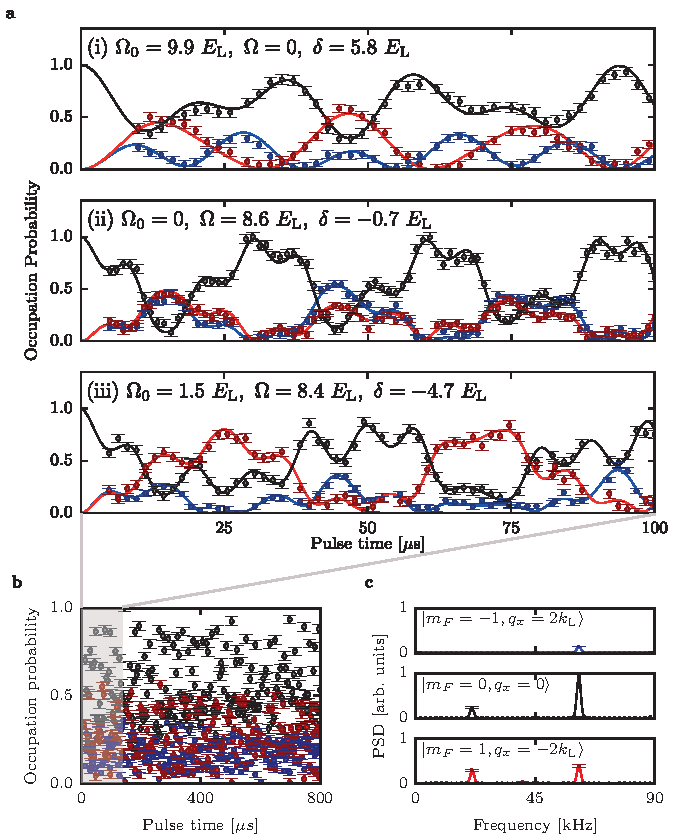
\includegraphics{Figures/Chapter5/Fig5.pdf}
		\caption[Time evolution and Fourier transforms of a SOC system]
		{{\bf a.}
		Occupation probability for the three states in the measurement basis $\ket{m_F=-1, q=q_x+2\kl}$ (blue), $\ket{m_F=0,q=q_x}$ (black), and $\ket{m_F=+1,q=q_x-2\kl}$(red),  following unitary evolution under $\hat{H}_{\mathrm{SOC}}$ for times up to 100 $\mu s$ at different spin-orbit coupling regimes: (i) $\Omega_0=9.9 E_{\mathrm{L}}$, $\Omega=04$,  $\delta=5.8 E_{\mathrm{L}}$, (ii) $\Omega_0=0$, $\Omega=8.6\,E_{\mathrm{L}}$,  $\delta=-0.7\,E_{\mathrm{L}}$, $\delta\omega=\epsilon+12\,E_{\mathrm{L}}$, and (iii) $\Omega_0=1.5\,E_{\mathrm{L}}$, $\Omega=8.4\, E_{\mathrm{L}}$,  $\delta=-4.7\,E_{\mathrm{L}}$, $\delta\omega=\epsilon+17\,E_{\mathrm{L}}$.
		{\bf b.} Occupation probability for long pulsing up to 800 $\mu$s for parameters as in (iii). 
		{\bf c.} Power spectral density of the occupation probability. We subtract the mean value of each probability before taking the Fourier transform to remove peaks at $f=0$. The peaks in the PSD then correspond to the relative eigenenergies of $\hat{H}_{SOC}$.
		}
		\label{fig:Figure5}
	\end{center}
\end{figure*}
%
We mapped the band structure of SOC atoms for three different coupling regimes. Figure~\ref{fig:Figure5}a shows representative traces of the measured occupation probabilities for short evolution times along with fits to the unitary evolution given by $\hat{H}_{\mathrm{SOC}}$ with $\delta$, $\Omega_0$, and $\Omega$ as free parameters. The fit parameters agree well with independent microwave and Raman power calibrations. In the lower two panels, where the Raman coupling strength was periodically modulated, the occupation probabilities oscillated with more than three frequencies since the full description of the system was given by a Floquet quasi-energy spectrum. Figure~\ref{fig:Figure5}b,c shows the occupation probabilities for the parameter regime (iii) for longer evolution times along with the PSD of the occupation probability of each spin state. 



\begin{figure}[!ht]
	\begin{center}
		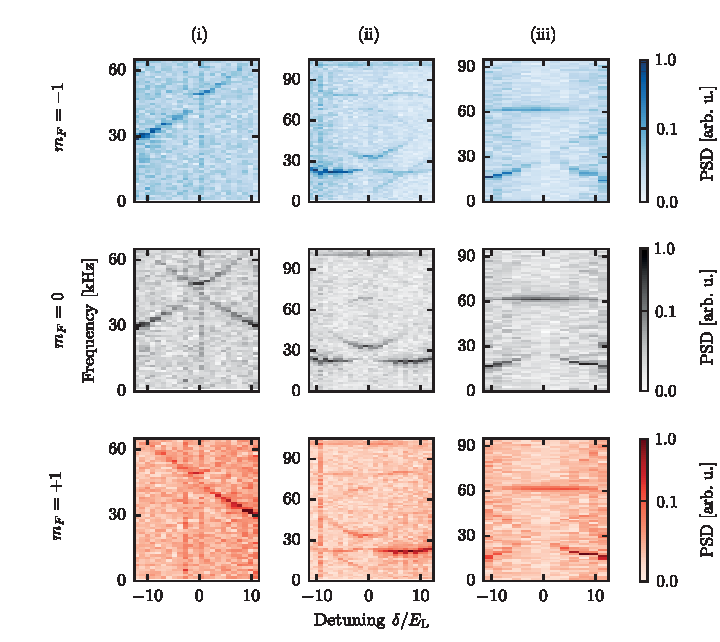
\includegraphics[width=4.8in]{Figures/Chapter5/Fig6a.pdf}
		\caption[Power spectral density of the time dependent occupation probability for each state in the measurement basis for three coupling regimes]
		{
			 Power spectral density of the time dependent occupation probability for each state in the measurement basis for three coupling regimes:
			{ (Left)} $\Omega_0=9.9 E_{\mathrm{L}}$, $\Omega=0$,
			{ (Center)} $\Omega_0=0$, $\Omega=8.6 E_{\mathrm{L}}$,  $\delta\omega=\epsilon+12 E_{\mathrm{L}}$, and
			{ (Right)} $\Omega_0=4.9 E_{\mathrm{L}}$, $\Omega=8.4 E_{\mathrm{L}}$,  $\delta\omega=\epsilon+17 E_{\mathrm{L}}$. Each panel is normalized to peak amplitude to highlight small amplitude features in the PSD of the periodically driven SOC, and the highest value on the frequency axis corresponds to the FFT bandwidth.
		}
		\label{fig:Figure6a}
	\end{center}
\end{figure}

We used a non-uniform fast Fourier transform algorithm (NUFFT) on a square window to obtain the power spectral density of the occupation probabilities since our data points were not always evenly spaced because of imperfect imaging shots. The heights of the peaks in the PSD are related to the magnitude of the overlap integrals between the initial state and the Raman dressed states. Figure~\ref{fig:Figure5}c shows the raw PSD of the time evolution of the system under $\hat{H}_{\mathrm{SOC}}$ for a given Raman coupling strength and detuning. We put together all the PSDs for the three coupling regimes in the spectra shown in Figure~\ref{fig:Figure6a}. Each column corresponds to a different coupling regime and the colors represent the different spin states of the measurement basis. The spectra show that some overlap integrals vanish near $\delta=0$, which is manifested as missing peaks in the PSD. The periodic structure of the Floquet quasi-energy spectrum gave rise to peaks at constant frequencies of $\delta\omega$ and $2\delta\omega$ independently of the Raman detuning, and a structure that is symmetric about the frequencies $2\pi f_1=\delta\omega/2$ and $2\pi f_2=\delta\omega$. A reader is interested in seeing another nice experiment where the Floquet quasienergy spectrum becomes can be visualized is advised to see~\cite{deng_observation_2015}.


\subsection{Effective mass}
\label{sec:effective_mass}

Fourier transform spectroscopy only gives access to the relative energies of a Hamiltonian. If we want to recover the absolute energies we need to have an additional energy reference. The particular Hamiltonian $\hat{H}_{SOC}$ had a ground state with a nearly quadratic dispersion. We measured its effective mass to obtain the ground state energy which we used as a reference to recover the absolute energies. 

We measured the effective mass of the Raman dressed atoms by adiabatically preparing the BEC in the lowest eigenstate and inducing dipole oscillations~\cite{Pethick}. The effective mass of the dressed atoms was related to the bare mass $m$ and the bare and dressed trapping frequencies $\omega$ and $\omega^{*}$ along the Raman recoil direction by the ratio $m^{*}/m=(\omega/\omega^{*})^2$. We measured this ratio following~\cite{lin_synthetic_2011}. To induce the oscillations we started in  $\ket{m_F=0,\, k_x=0}$ state and adiabatically turned on the Raman laser in $10\,\mathrm{ms}$ while simultaneously ramping the detuning to $\delta\approx0.5\,\El$ which shifted the minima in the ground state energy away from zero quasi-momentum. We suddenly brought the field back to resonance causing an abrupt change in the dispersion relation that excited the dipole mode of the BEC. To obtain the bare state $\omega$ we only used the Raman beams to induce the oscillations and then subsequently turned off the beams while the BEC oscillated in the dipole trap and to obtain $\omega^*$ the Raman beams were kept on the whole time.
For this set of measurements, we adjusted our optical dipole trap to give new trapping frequencies $(\omega_x, \omega_y, \omega_z)/2\pi=(35.6(4), 32.2(3), 133(3))\,\Hz$, nominally symmetric in the plane defined by $\ex$ and $\ey$. 

The Raman beams were co-propagating with the optical dipole trap beams; therefore, the primary axes of the dipole trap frequencies were at a $45^{\circ}$ angle with respect to the direction of $\mathbf{k}_{\mathrm{L}}$. The kinetic and potential terms in the Hamiltonian including the contribution of the Raman and optical dipole trap were

\begin{align}
\hat{H}_{\perp}= &\frac{\hbar^2q_x^2}{2m^{*}} + \frac{\hbar^2q_y^2}{2m}+\frac{m}{2}[\omega_{x'}^2x'^2+\omega_y'^2y'^2] \nonumber \\
= & \frac{\hbar^2}{2m^{\star}}k_x^2 + \frac{1}{2m}k_y^2+\frac{m}{4}[(\omega_{x'}^2+\omega_{y'}^2)(x^2+y^2)+2xy(\omega_{x'}^2-\omega_{y'}^2)],
\end{align}
%
where $x'=(x+y)/\sqrt{2}$ and  $y'=(x-y)/\sqrt{2}$ are position coordinates rotated by $45^{\circ}$ . For an axially symmetric trap with $\omega_{x'}=\omega_{y'}$, the frequency of oscillation along the Raman recoil direction  is 

\begin{equation}
\omega_x^2=\frac{m}{2m^{*}}(\omega_{x'}^2+\omega_{y'}^2).
\label{Eq:meff}
\end{equation}

Our trap had a small $3.4$\,Hz asymmetry and there was some coupling of the motion along the axis perpendicular to $\k_{\rm L}$ which becomes more significant at larger values of the effective mass. The sampling times for the measurements were small compared to the trap asymmetry and we can locally approximate the motion of the atoms by a simple harmonic function with a frequency along $\ex$ given by Equation~\ref{Eq:meff}.

Figure~\ref{fig:Figure4} shows the dipole oscillations along the $\mathbf{e}_{x}$ and $\mathbf{e}_{y}$ directions for the three different coupling regimes we explored, as well as the bare state motion. The resulting mass ratios for the three coupling regimes are $m/m^{*}=$  (i) $1.04(8)$, (ii) $0.71(7)$, and (iii) $0.62(4)$.
\begin{figure*}[!ht]
	\begin{center}
		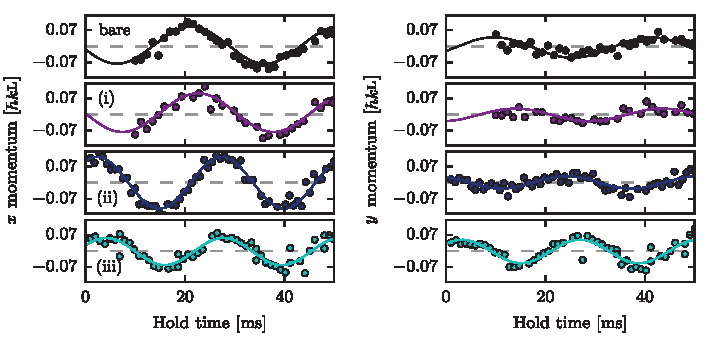
\includegraphics{Figures/Chapter5/Fig4.pdf}
		\caption[Dipole oscillations of a spin-orbit coupled BEC in a dipole trap]
		{  Oscillation of the BEC in the dipole trap along the  recoil directions $\mathbf{e}_{x}$ and  $\mathbf{e}_{y}$ for (top) bare atoms, and the three parameter regimes that we explored (i), (ii), and (iii).  We believe that the observed low amplitude oscillations along $\ey$ are due to the initial detuning ramp not being fully adiabatic. 
		\label{fig:Figure4}}
	\end{center}
\end{figure*}

\subsection{Measured dispersions}

Figure \ref{fig:Figure7} explains in detail the interpretation of the multiple peaks in the PSD and the steps that were taken to recover the dispersion relation using the effective mass and the Fourier spectra. The red line in Figure~\ref{fig:Figure7}a represents a level within a Floquet manifold that has the largest overlap integral with the initial $\ket{m_F=0, q=0}$ state. The peaks in the PSD correspond to energy differences between the marked level and the levels in neighboring Floquet manifolds pointed by the colored arrows. We show the theoretically computed energy differences on top of the measured PSD in panel b. The lowest frequency dominant peaks of the PSD correspond to energy differences with the adjacent lower Floquet manifold. To properly recover the SOC dispersion we shifted the PSD by a negative quadratic term $-\hbar^2q_x^2/2m^{*}$ as we show on panel c. We finally invert the frequency axis and shift it by $\delta\omega$. %Including the effective mass to reconstruct the spectrum of the time-independent SOC case, amounts to shifting the PSD by a positive quadratic term.
\begin{figure*}[!ht]
	\begin{center}
		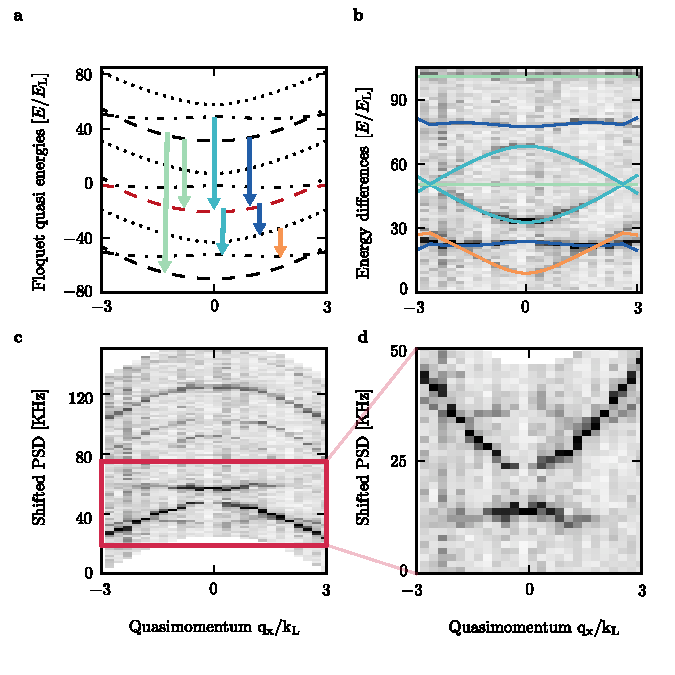
\includegraphics{Figures/Chapter5/Fig7.pdf}
		\caption[Converting energy differences into absolute energies]
		{  {\bf a} Floquet quasi-energy spectrum of a SOC Hamiltonian with periodic coupling strength. The red line represents the eigenstate that has the largest overlap with the initial $\ket{m_F=0}$ state. The arrows indicate the energies of the states that have non-zero overlap with the initial state and can be measured with Fourier transform spectroscopy.
		{\bf b} PSD of the occupation probability and numerically calculated energy differences between the levels indicated by the arrows on panel a.
		{\bf c} PSD shifted by a quadratic term $-\hbar^2 q^2_x/2m^*$. The red box indicates the region of interest where we can recover the SOC spectrum.
		{\bf d} We invert the frequency axis and shift it by $\delta\omega$.   
		}
		\label{fig:Figure7}
	\end{center}
\end{figure*}

We obtained the characteristic dispersion of a SOC system after adding a quadratic term to the PSD, proportional to the measured effective mass and rescaling the detuning into recoil momentum units. We combined the PSD of the time evolution of the three $\ket{m_F}$ states to look at the spin dependence of the spectra. Figure \ref{fig:Figure6b} shows the measured dispersion relations as well as the Floquet quasi-energies calculated for the Hamiltonian parameters obtained from our calibrations. The spectral lines that can be resolved with our technique depend on the overlap integrals of the initial state with the target Hamiltonian eigenstates. Additional energies can be measured by repeating the experiment with different initial states. The spectral lines we were able to resolve are in good agreement with the calculated energies of the Hamiltonian. 
\begin{figure}[!ht]
	\begin{center}
		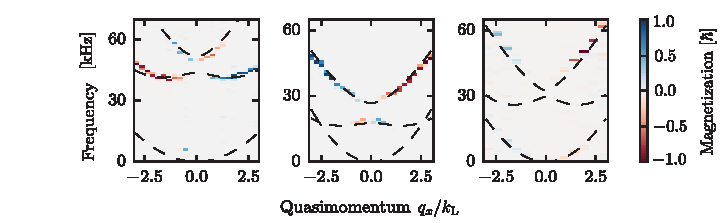
\includegraphics{Figures/Chapter5/Fig6b.pdf}
		\caption[Spin-dependent SOC dispersion for three different coupling regimes]
		{
			Spin-dependent SOC dispersion for three different coupling regimes. We combine the PSD of the occupation probability of the states $\ket{m_F=\pm 1, q_x=\mp 2k_{\mathrm{L}}}$, and shift each frequency by an amount proportional to the squared quasimomentum and the effective mass. The dashed lines are the calculated Floquet energies for the Hamiltonian using our calibration parameters. 
		}
		\label{fig:Figure6b}
	\end{center}
\end{figure}


\section*{Conclusion}

This chapter introduced the basic principles of the Fourier transform spectroscopy technique and used it to measure the spin and momentum dependent dispersion relation of a spin-1 spin-orbit coupled BEC. We additionally studied a periodically driven SOC system and found a rich Floquet quasi-energy spectrum. Our method can be applied generically to any system with long enough coherent evolution to resolve the energy scales of interest and could prove particularly useful to study systems where it is harder to predict or compute the exact energies, such as cold atom realizations of disordered or highly correlated systems \cite{eisert_quantum_2015}. In our lab, this technique has been used to study the spectrum of a Rashba spin-orbit coupled system~\cite{valdes-curiel_unconventional_2019} and of a fractional period adiabatic superlattice~\cite{anderson_realization_2019}.

Our main initial interest was to create tunable spin-orbit coupling and Fourier spectroscopy was conceived as a tool to characterize it. We realized that the use of Raman transitions from multiple frequency beams was equivalent to another experiment that achieved tunable SOC using amplitude modulated Raman coupling~\cite{jimenez-garcia_tunable_2015}.  %We therefore decided to focus on Fourier spectroscopy instead, a decision that turned out to be very fruitful for our lab as we continue to use this technique to characterize the spectrum of a variety of systems. 

% The idea of Fourier transform spectroscopy was born from a very different natured project. The project was originally conceived as a way to engineer tunable spin-orbit coupling using multiple-tone Raman transitions. The inspiration came from a previous project where we used multiple-tone Raman transitions to engineer a spin-1 spin-orbit coupled system whose ground state presented different magnetic phases~\cite{campbell_magnetic_2016}. Fourier spectroscopy was conceived as a new way to characterize the tunable dispersion relation resulting from our proposed coupling scheme. Unfortunately, we realized that this proposal was equivalent to another experiment that achieved tunable SOC using amplitude modulated Raman coupling~\cite{jimenez-garcia_tunable_2015}. We therefore decided to focus on studying Fourier spectroscopy instead, a decision that turned out to be very fruitful for our lab as we continue to use this technique to characterize the spectrum of a variety of systems. 







